\section{Introduction}\label{sec:introduction}

%- Serverless cloud computing and the Function-as-a-Service (FaaS) execution
%  model have become popular for managing large applications due to their
%  operational benefits and pay-as-you-go billing model.
%- FaaS (Function-as-a-Service) boosts developer productivity by managing
%  operational tasks and allowing developers to focus on writing code.
%- FaaS has become a popular cloud execution model supported by major cloud
%  providers and allows for elastic, scalable, and event-driven applications.
%- FaaS is utilized in various contexts, including in data centers with private
%  FaaS platforms and in High Performance Computing to manage supercomputers more
%  efficiently.

\IEEEPARstart{S}{erverless} cloud computing and the Function-as-a-Service (FaaS)
execution model are increasingly favored for administering large-scale
applications given their operational advantages and pay-as-you-go billing model
\cite{hendrickson2016serverless, bermbach2021future}. Widely supported by
leading cloud providers, FaaS inherently boosts developer productivity by
assuming responsibility for operational tasks, thus allowing developers to
channel more focus into code writing \cite{bermbach2021future}. FaaS, designed
for compatibility with elastic, scalable, and event-driven applications, is
employed in an array of contexts \cite{eismann2020serverless,
hendrickson2016serverless}. Notably, it is used within data centers through
private FaaS platforms \cite{eismann2020review} and in the realm of High
Performance Computing, bringing about more efficient supercomputer management
\cite{spillner2018faaster, chard2020funcx}.

% But there are also challenges. Possibly high costs due to double billing:
% through synchronous function calls, called function costs incurred, waiting
% function billed though not doing work. Double billing illustrated in Figure
% \ref{fig:doublespending}. High latencies through cascading cold starts:
% overhead of creating a new function instance on demand, Cold start accumulates
% in FaaS compositions with chains of functions, executing in sequence Increases
% end-to-end latency and execution cost of application, shown in Figure
% \ref{fig:cascading_cold_start}. High latencies through HTTP requests instead
% of local function calls: FaaS platforms designed for function invocation over
% network HTTP requests used, considerable invocation overhead for internal
% function calls. Possibly inefficient resource utilization (e.g., during
% request spikes): both synchronous and asynchronous calls are executed
% immediately, although async functions could be delayed.

Nevertheless, there are several challenges in the context of FaaS platforms that
need to be addressed. Among these is the possibility of incurring high costs due
to double billing. This occurs when synchronous function calls are charged, thus
creating costs for both the called function \emph{and} the waiting function,
even if it is not carrying out any work \cite{baldini2017serverless}. This
concept is illustrated in Figure \ref{fig:doublespending}. Added to this, there
may be high latencies caused by cascading cold starts, which refers to the
process of on-demand creation of a new function instance when there is a change
in the load or when existing instances are otherwise engaged. When such cold
starts accumulate in FaaS compositions with chains of functions, executing in
sequence, it can significantly increase the end-to-end latency and the execution
cost of the application \cite{bermbach2020using, daw2020xanadu}. This is shown
in Figure \ref{fig:cascading_cold_start}. There can also be high latencies due
to the use of HTTP requests instead of local function calls. FaaS platforms are
designed for function invocation over network, resulting in a significant
invocation overhead for internal function calls \cite{jia2021nightcore,
qi2022spright}. Furthermore, in the context of FaaS, two types of function
invocation methods exist -- synchronous, where the caller waits for the outcome,
and asynchronous, where the caller does not. Immediate execution is currently
the norm with both these invocation methods. However, their impact on resource
utilization varies. In scenarios like request spikes, immediate execution of
both synchronous and asynchronous calls can lead to inefficient resource
utilization. Immediate execution for synchronous calls is necessary to provide
an immediate response as per the caller's demand. Conversely, asynchronous
function calls do not require immediate execution, presenting the opportunity to
delay execution and thereby offering increased flexibility in scheduling
operations \cite{schirmer2023profaastinate}.

\begin{figure}
    \centering
    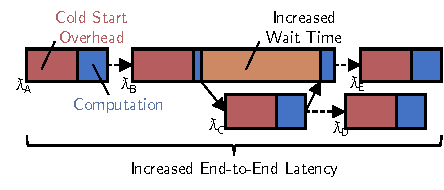
\includegraphics[width=.9\linewidth]{../figures/cascadingcoldstart}
    \caption{
        Cold start cascades refer to a sequence of first-time function
        executions, such as during changes in load. The cumulative cold start
        overhead from each instance extends the overall latency and waiting
        periods for synchronous executions. \cite{bermbach2020using}.
    }
    \label{fig:cascading_cold_start}
\end{figure}

\begin{figure}
    \centering
    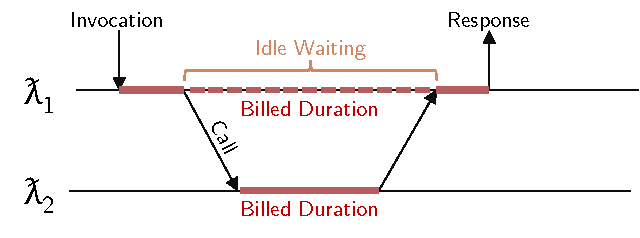
\includegraphics[width=\linewidth]{../figures/doublespending}
    \caption{
        Invoking functions synchronously in the duration-based billing model of
        FaaS might result in duplicate charges: both lambda functions can incur
        expenses when ${\lambda}_{1}$ calls on ${\lambda}_{2}$ due to idle
        waiting times and call overheads \cite{schirmer2023fusionize}.
    }
    \label{fig:doublespending}
\end{figure}

%- Schirmer et al. addresses these issues with FUSIONIZE , a framework that
%  automates the optimization of multi-function application compositions in
%  serverless computing by fusing application code into an optimized
%  multi-function composition.
%- Use the concept of function fusion to expand remote FaaS function calls with
%  task source code where beneficial, eliminating remote call overheads and
%  restricting cold start cascades.
%- Optimize the infrastructure configuration of deployed functions, including
%  allocated memory and CPU shares, without requiring additional configuration or
%  application descriptions from developers.
%- Infer the call patterns, cost efficiency, and performance from live execution
%  behavior of existing FaaS applications, and iteratively optimize the
%  application deployment for cost efficiency and end-to-end performance.
%- Automatically adapt to changes in application behavior or environment to
%  continuously optimize deployment for further cost efficiency and performance
%  improvements.

Schirmer et al. addresses the issues of cascading cold starts, double billing
and remote function invocation overhead with \textsc{Fusionize}
\cite{schirmer2023fusionize}, a framework aimed at auto-optimizing
multi-function application compositions in serverless computing.
\textsc{Fusionize} employs function fusion, expanding remote FaaS calls with
task source code when beneficial, reducing remote call overheads and avoiding
cold start cascades. The infrastructure configuration is optimized autonomously
to avoid further developer input. \textsc{Fusionize} also analyzes patterns,
efficiency, and performance from the real-time usage of FaaS applications to
consistently improve deployment for cost and performance. Importantly, the
framework can adapt to changes in the application or its environment ensuring
ongoing optimization.

Akkus et al. rival Schirmer's approach with the serverless computing system SAND
through application-level sandboxing and a hierarchical message bus
\cite{akkus2018sand}. This system enables two distinct levels of isolation: one
among multiple applications and another between functions of the same
application. This ensures efficient use of cloud resources and reduces startup
latency. SAND's hierarchical structure for message queuing and storage leverages
locality for function interaction and data sharing within applications. It uses
local and global message buses for fast processing and reliability. SAND
achieves low latency in function interaction and startup while improving
resource efficiency, making it particularly fitting for resource-limited edge
data centers.

% -  Schirmer et al. presents a system called ProFaaStinate which allows
%    serverless platforms to delay the execution of function calls until a time
%    when resources are abundantly available.
% - This approach is applicable to asynchronous calls where immediate execution
%   of functions is not a requirement.
% - By delaying function execution to periods of low load, the observable
%   latency of synchronous requests can be decreased, spreading resource usage
%   over a longer time.
% - The proposed solution is designed to take advantage of load and resource
%   fluctuations in Function-as-a-Service (FaaS) platforms.
% - It does not require complex systems modelling, scheduling mechanisms, or
%   load prediction techniques.
% - The system is evaluated by implementing it on top of the Nuclio open-source
%   serverless platform.

Finally, in discussing the issue of inefficient execution of synchronous and
asynchronous function calls, Schirmer et al. presents \textsc{ProFaaStinate}
which enhances serverless platforms by delaying the execution of function calls
until resources are abundant \cite{schirmer2023profaastinate}. This method is
especially applicable to asynchronous calls, where immediate execution is not
absolutely necessary. By allowing the function execution to be delayed until
periods of low load, the observable latency of synchronous requests is reduced.
This spreads the usage of resources over an extended period preventing any
bottleneck situations. \textsc{ProFaaStinate} benefits from load and resource
fluctuations which are a common occurrence in FaaS platforms. This approach
stands out as it does not call for any intricate systems modelling, scheduling
mechanisms, or load prediction techniques. The approach's validity is confirmed
through a proof-of-concept implementation on Nuclio, an open-source serverless
platform\footnote{\url{https://nuclio.io/}}.


% Following the example of \textsc{ProFaaStinate}, in scope of this project we
% implement the concepts of the three approaches within Nuclio to showcase
% optimization opportunities of provider-side access to serverless platforms.
% We hope to create a system that can overcome these common challenges in FaaS
% platforms and inspires future research and commercial implementations.

Within the scope of this project, we aim to follow the prototype set by
\textsc{ProFaaStinate}. Our goal is to implement the concepts from the three
approaches within Nuclio as a means to expose potential avenues for optimization
from the provider's perspective in serverless platforms. We aspire to design a
system capable of overcoming these common challenges often encountered in FaaS
platforms as a whole. Through our initiative, we hope to encourage further
research and provider-side implementations in this field.


